\documentclass[11pt]{article}

\usepackage[margin=1in]{geometry}
\usepackage{graphicx}
\usepackage{verbatim}
\usepackage{listings}



\title{Distributed Graph Processing for Machine Learning:\\
The Case for Condor and Spot Instances}
\author{Jing Fan~~~~~Ce Zhang}
\date{}

\begin{document}
\maketitle

\begin{abstract}
We study distributed graph processing for machine learning
applications in an environment
in which the failure of workers is guaranteed to happen
frequently. Notable examples of such environments can be found
both in the classic grid computing, e.g., Condor, and the emerging
cloud computing, e.g., {\em spot instances} on Amazon EC2.
Different from the common practice that running
machine learning algorithms with a dedicated cluster,
it is still an open research question that how (and whether
it is possible) to run machine learning algorithms in
this environment.

This report documents our {\em preliminary} effort towards 
answering this question by building a prototype system. 
Ideally, we have two goals: (1) {\em expressiveness}:
this prototype system should allow the user to specify
a machine learning system as easy as existing frameworks
designed for dedicated clusters; and (2) {\em efficiency}:
the machine learning system specified by the prototype system
should be able to run in environments such as Condor efficiently.
We report our design of this prototype system that extends
the programming model of a popular graph-processing engine,
namely GraphLab. Given a user program written in our language
extension, we describe the execution model. We validate
our prototype system with an emergingly popular machine
learning application, namely deep neural network, on {\em both}
Condor and Amazon EC2. We find that our prototype system is
able to achieve more than 12TFLOPS on Condor with more than
2.6K cores harvest from the national Open Science Grid (OSG).

\end{abstract}

\section{Introduction}

Machine learning has been one emerging area that
attracts interests from the community of system 
research, especially research of 
distributed systems~\cite{Li:2014:OSDI,GraphLab:OSDI}. 
Notable example including GraphLab~\cite{GraphLab:OSDI},
Spark~\cite{Spark}, Google's DistBelief~\cite{Google}, and 
Yahoo's Parameter Server~\cite{Yahoo,Li:2014:OSDI}. 
In this work, we focus on the same goal, that is 
to build a framework that supports executing machine 
learning applications in an distributed environment.

It has been a common practice for distributed machine
learning systems to be run on dedicated clusters.
For example, both Spark and GraphLab has been 
reported to be able to execute machine learning algorithms
on hundreds of machines; DistBelief is able to 
train deep neural network on 6000 machines; and 
Parameter Server is able to scale to 1000 machines.
Our key observation is that existing frameworks~\cite{Li:2014:OSDI,
GraphLab:OSDI,Spark,Google,Yahoo} implicitly
make {\em at least one} of the following two assumption
about the distributed environment and workload:

\begin{enumerate}
\item The coordinators know {\em a priori} 
the set of worker nodes, including their configuration,
number of worker nodes, and the network topology between
these workers. These information are necessary for most
existing systems to schedule their workload before
execution. For example, Yahoo's Parameter Server
uses consistent hashing~\cite{Li:2014:OSDI} to allocate
resources and workers, and use chain replication to
deal worker failures. GraphLab~\cite{GraphLab:OSDI} also
uses similar approaches. 
\item The graph to be processed consists of nodes that are 
executed with the same level of consistency. For example,
in GraphLab, the execution engine can choose from three
different consistency levels, and all the nodes in the same
graph will follow the same level.  
\end{enumerate}

These assumptions are often true in the environment that
these systems are designed for, in which the cluster is
maintained in a centralized way or leased with cloud-based
services (e.g., EC2). However, this assumption
does not always hold for a popular environment that
often be called {\em high throughput computation} (HTC) 
environment. One notable example is Condor, which,
when ran on the national open science grid, can easily
harvest hundreds of thousands of machine hours per day.
Another example is the spot instance on Amazon EC2, which 
relies on a bidding-based model that could provide much
cheaper solution than traditional cloud-based instances.
These HTC environments have the characteristics that are
different to the above two assumptions when applied to 
machine learning.

\begin{enumerate}
\item The coordinators does not know the set of workers
{\em a priori}. For example, in Condor, the coordinator
does not know how many workers will be assigned to it, and
what type of machines will be assigned to it. Also, the
workers are not guaranteed to be able to communicate with each
other. Similar scenario applies to spot instances
of EC2, in which the number of workers assigned to the
coordinator depends on the bidding price and other bidder, while
the configuration of machines are known to the coordinator.
\item Machine learning workload often contains heterogeneous
consistency requirement. For example, for some data
in machine learning workload, full consistency is not required,
while for other data, one might need higher-level of consistency.
This observation has also been made in a subset of
existing systems, e.g., Parameter Server~\cite{Li:2014:OSDI}.
\end{enumerate}

We study how to build a GraphLab-like system with these two
observations, and study their implications on system design.
We first propose a language extension of GraphLab for the
user to specify a machine learning algorithm, and use
Deep Neural Network (DNN) as an use case. We then study
the design decisions we made for both Condor and spot
instances of Amazon EC2. We validate our prototype system
on standard benchmark data sets.

\section{System Design}

We describe the design decisions and how they relate to
the two observations we made on Condor and spot
instances of Amazon EC2. We first describe in more details
about these environment, and present the language extension
and execution model.

\begin{figure}[t]
\centering
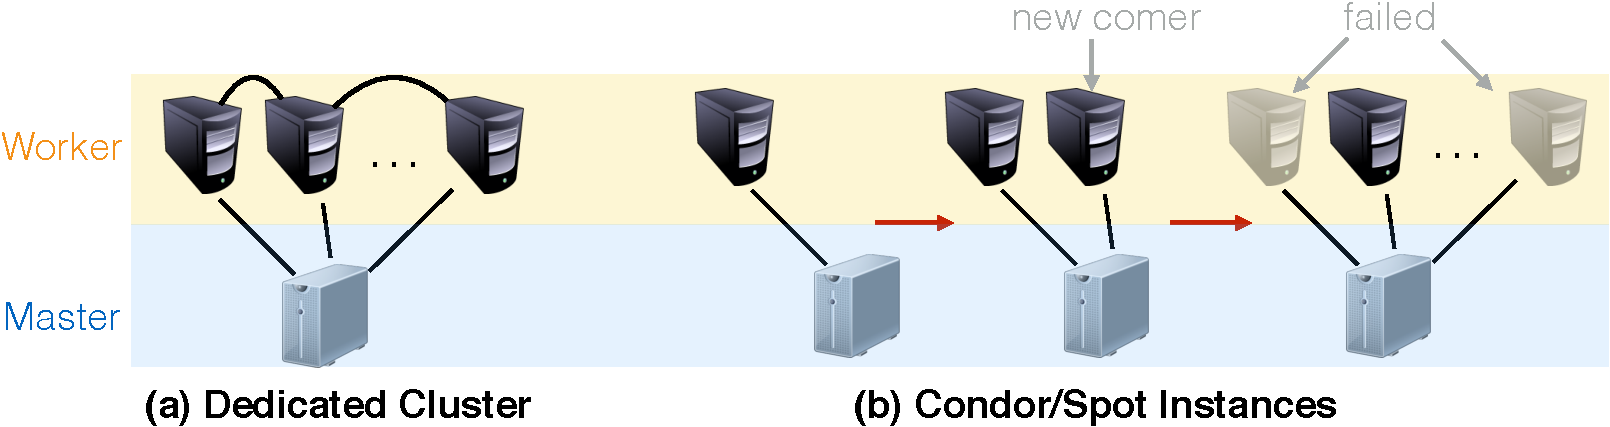
\includegraphics[width=0.9\textwidth]{figures/env-crop}
\caption{An illustration of (a) dedicated cluster and (b) Condor/Spot-instances. (b) illustrates three states in different time where the worker machines keeps come in and fail.}
\label{fig:env}
\end{figure}

\subsection{Condor and Spot Instance of EC2}

Figure~\ref{fig:env} illustrates the difference between
a dedicated cluster, Condor instances, and EC2 instances.
We describe their difference as follows.

\paragraph*{Dedicated Cluster}


\paragraph*{Condor}


\paragraph*{EC2 Spot Instances}


\subsection{User Interface}
\subsubsection{Language Extension}

\subsubsection{Vertex-centric APIs}
A vertex in the graph is modeled by the \textsf{Vertex} data structure:
\begin{verbatim}
class Vertex {
  NodeIdType nodeId;
  T data;
  vector<Vertex> neighbours;
};
\end{verbatim}
We expose baisc operations of a vertex, including viewing and updating the 
value of itself and its neighbours. The APIs are shown in 
Table~\cite{table:api}. The APIs enable programmers to make queries 
from the perspective of a vertex (in a vertex-centric way). 
\begin{table}
  \centering
 \begin{tabular}{|c|c|}
 \hline
 \hline
 Function & Usage\\
 NodeIdType getNodeId() & Get the id of this vertex.\\
 VertexData$\langle$T$\rangle$ getData() & Get the data of this vertex.\\
 void getNeighbours(vector$\langle$Vertex$\langle$T$\rangle$ $\rangle$\& 
neighbours) & Get all the neighbour information.\\
 void updateValue(NodeIdType nodeId, VertexData$\langle$T$\rangle$ val) & Update 
the value of vertex nodeId to val.\\
 \hline
 \hline
 \end{tabular}
 \caption{APIs and Usage}
 \label{table:api}
\end{table}

\subsubsection{Example of Deep Neural Network for Image Recongnition}
We illustrate the usage of the system by the example of deep	neural	network	
for image recognition. In the \textbf{DNN}, we have two kind of vertices, one 
being the vertex that stores the real image data and the other being the neural 
network vertex that contains the parameters to learn. 
We define \textsf{f.cpp} for the image vertices and \textsf{g.cpp} for the 
"averagble" neural netowrk vertex, as shown in Listing~\ref{lst:f}~\ref{lst:g}.
\begin{lstlisting}[language=java,basicstyle={\ttfamily\small},caption={f.cpp},label={lst:f},frame=single]
 int main(){ 
   // get vertex content
   Image *img = getData<Image>();
   // get neighbors’ content 
   vector<Node> neighbours = getNeighbours(); 
   Network *nw = getData<Network>(&neighbours[0]); 
   NodeId nwId = nw.nodeId;
   // do training of neural network
   Layer *layer1 = nw->layers[0];
   Layer *layer6 = nw->layers[5];
   layer6->ops[0]->label = img->label; for (int i = 0; i < 4; ++i) {
   layer1->ops[i]->inputs[0] = img->content; }
   nw->forward();
   nw->backward();
   // write back new content 
   updateValue<Network>(nwId, nw);
 }
\end{lstlisting}
\begin{lstlisting}[language=java,basicstyle={\ttfamily\small},caption={g.cpp},label={lst:g},frame=single]
 int main(){ 
   // get two replicas 
   Network *nw1 = getData<Network>(); 
   Network *nw2 = getData<Network>();
   // do the average 
   nw1->avg_with(nw2); 
   nw2->copy_from(nw1);
   // write back new content 
   updateValue<Network>(getNodeId(), nw1);
 } 
\end{lstlisting}

\subsection{Execution Model}
We have two kinds of vertices and also two kinds of workers. 
\section{Performance Study}

\bibliographystyle{abbrv}
\bibliography{report}

\end{document}


















